% 原分章PDF第46页7.1.5.3标题至第50页7.1.5.4标题前。
\subsubsection{用于因果推断的距离相关}
距离相关可以用来检验原因与因果生成机制之间的独立性。考虑$p$维随机向量$X$与$q$维随机向量$Y$，以$P(X,Y)$表示二者的联合分布。分别以$P(X)$和$P(Y\mid X)$表示$X$的密度函数，以及给定$X$时$Y$的条件密度函数；类似地可以定义$P(Y)$与$P(X\mid Y)$。关联分析度量的是两个随机向量之间的依赖性，而因果分析度量的是两个分布之间的依赖性。

\begin{bookdefinition}{7.10}
\textbf{原因与效应之间的距离相关度量。}两个分布之间的距离相关依赖性度量定义为
\begin{equation}
\Delta_{X\to Y}=R\bigl(P(X),P(Y\mid X)\bigr),\tag{7.181}
\end{equation}
\begin{equation}
\Delta_{Y\to X}=R\bigl(P(Y),P(X\mid Y)\bigr).\tag{7.182}
\end{equation}
\end{bookdefinition}
假设将$X$与$Y$分别离散化（或划分）为$m$组与$k$组。令$m_i$为$X$落入第$i$组的点数，$k_{ij}$为$X$落入第$i$组且$Y$落入第$j$组的点$(X,Y)$的个数。于是$n=\sum_{i=1}^m m_i$，$m_i=\sum_{j=1}^k k_{ij}$。令$X^{(i)}$为第$i$组中所有$X$点的集合，$Y^{(j)}$为第$j$组中所有$Y$点的集合。密度函数$P(X^{(i)})$的估计为$P(X^{(i)})=m_i/n$，条件密度函数为$P(Y^{(j)}\mid X^{(i)})=k_{ij}/m_i$。

\begin{bookexample}{7.13}
考虑两个向量$X$和$Y$，将各向量的每个分量离散化（或划分）为两类。因此，$X$与$Y$可写为（图7.3）
\[
X=[X_1\ X_2]=\begin{bmatrix}x_{11}&x_{12}\\x_{21}&x_{22}\end{bmatrix},\qquad
Y=[Y_1\ Y_2]=\begin{bmatrix}y_{11}&y_{12}\\y_{21}&y_{22}\end{bmatrix}.
\]
$X$与$Y$各分为四组：
\[
\begin{aligned}
X^{(1)}&=(x_{11},x_{12}),&X^{(2)}&=(x_{11},x_{22}),\\
X^{(3)}&=(x_{21},x_{12}),&X^{(4)}&=(x_{21},x_{22}),
\end{aligned}
\]
以及
\[
\begin{aligned}
Y^{(1)}&=(y_{11},y_{12}),&Y^{(2)}&=(y_{11},y_{22}),\\
Y^{(3)}&=(y_{21},y_{12}),&Y^{(4)}&=(y_{21},y_{22}).
\end{aligned}
\]
图7.3表明，$X$与$Y$共同组成16组。概率密度与条件概率密度函数向量定义为
\[
P(X^{(i)})=\frac{m_i}{n},\quad i=1,2,3,4,
\]
以及
\[
P(Y^{(j)}\mid X^{(i)})=\frac{k_{ij}}{m_i},\quad i=1,\ldots,4,\quad j=1,\ldots,4.
\]
类似地可以计算$P(Y)$和$P(X\mid Y)$。
\end{bookexample}
\begin{figure}[htbp]
\centering

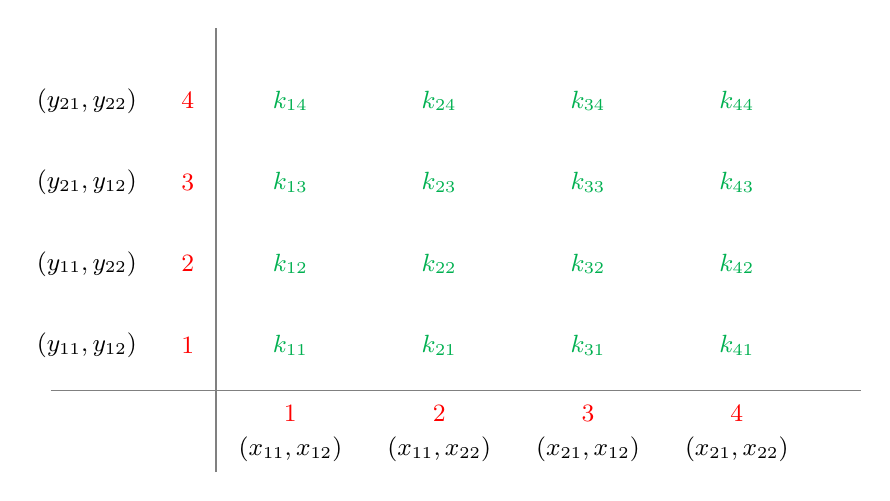
\begin{tikzpicture}[x=2.1cm,y=1.15cm,font=\small]
\definecolor{chSevenADGridGreen}{RGB}{0,176,80}
\draw[gray,line width=.5pt] (-1,0)--(3.9,0);
\draw[gray,line width=.5pt] (0,-.9)--(0,4.0);
\foreach \i in {1,2,3,4}{
  \foreach \j in {1,2,3,4}{
    \node[text=chSevenADGridGreen] at ({.45+.9*(\i-1)},{.5+.9*(\j-1)}) {$k_{\i\j}$};
  }
  \node[text=red] at ({.45+.9*(\i-1)},-.25) {$\i$};
  \node[text=red] at (-.17,{.5+.9*(\i-1)}) {$\i$};
}
\node at (.45,-.65) {$(x_{11},x_{12})$};
\node at (1.35,-.65) {$(x_{11},x_{22})$};
\node at (2.25,-.65) {$(x_{21},x_{12})$};
\node at (3.15,-.65) {$(x_{21},x_{22})$};
\node[anchor=east] at (-.42,.5) {$(y_{11},y_{12})$};
\node[anchor=east] at (-.42,1.4) {$(y_{11},y_{22})$};
\node[anchor=east] at (-.42,2.3) {$(y_{21},y_{12})$};
\node[anchor=east] at (-.42,3.2) {$(y_{21},y_{22})$};
\end{tikzpicture}

\origfig{3}{将数据组织为分组。}
\end{figure}

下面研究距离相关的计算。定义
\begin{equation}
\alpha_i=P(X^{(i)}),\quad i=1,\ldots,m,\tag{7.183}
\end{equation}
\begin{equation}
\begin{aligned}
\beta_i&=\bigl[P(Y^{(1)}\mid X^{(i)}),\ldots,P(Y^{(k)}\mid X^{(i)})\bigr]^T\\
&=[\beta_{i1},\ldots,\beta_{ik}]^T,\quad i=1,\ldots,m.
\end{aligned}\tag{7.184}
\end{equation}
再定义
\begin{equation}
\begin{aligned}
a_{ij}&=|\alpha_i-\alpha_j|,\quad
a_i=\frac1m\sum_{j=1}^m a_{ij},\quad
a_{.j}=\frac1m\sum_{i=1}^m a_{ij},\\
a_{.,}&=\frac1{m^2}\sum_{i=1}^m\sum_{j=1}^m a_{ij},
\end{aligned}\tag{7.185}
\end{equation}
\[
b_{ij}=\|\beta_i-\beta_j\|_2
=\sqrt{(\beta_{i1}-\beta_{j1})^2+\cdots+(\beta_{ik}-\beta_{jk})^2},
\]
\[
\begin{aligned}
b_{i.}&=\frac1m\sum_{j=1}^m b_{ij},\quad
b_{.j}=\frac1m\sum_{i=1}^m b_{ij},\\
b_{..}&=\frac1{m^2}\sum_{i=1}^m\sum_{j=1}^m b_{ij},
\end{aligned}
\]
\begin{equation}
A_{ij}=a_{ij}-a_{i.}-a_{.j}+a_{..},\tag{7.186}
\end{equation}
\begin{equation}
B_{ij}=b_{ij}-b_{i.}-b_{.j}+b_{..},\quad i=1,\ldots,m,\quad j=1,\ldots,m.\tag{7.187}
\end{equation}
令$S_{X\to Y}=a_{..}b_{..}$。距离协方差定义为
\begin{equation}
V_m^2\bigl(P(X),P(Y\mid X)\bigr)
=\frac1{m^2}\sum_{i=}^{m}\sum_{j=1}^{m}A_{ij}B_{ij}.\tag{7.188}
\end{equation}
类似地，可以定义$V_m^2(P(Y),P(X\mid Y))$和$S_{Y\to X}$。定义
\begin{equation}
\Delta_{X\to Y}=\frac{mV_m^2\bigl(P(X),P(Y\mid X)\bigr)}{S_{X\to Y}},\tag{7.189}
\end{equation}
\begin{equation}
\Delta_{Y\to X}=\frac{mV_m^2\bigl(P(Y),P(X\mid Y)\bigr)}{S_{Y\to X}}.\tag{7.190}
\end{equation}
检验的零假设为$H_0$：两个向量$X$与$Y$之间不存在因果关系。检验二者因果关系的统计量定义为
\begin{equation}
T_C=|\Delta_{X\to Y}-\Delta_{Y\to X}|.\tag{7.191}
\end{equation}
当$T_C$较大时，或者有$\Delta_{X\to Y}>\Delta_{Y\to X}$，表示$Y$导致$X$；或者有$\Delta_{Y\to X}>\Delta_{X\to Y}$，表示$X$导致$Y$。当$T_C\approx0$时，则无法作出因果判定。

为了更准确地评估因果关系并计算检验的$P$值，需要求出零假设成立时检验统计量的抽样分布。然而，统计量$T_C$的分布尚无已知的解析计算式。置换检验提供了一种简便方法，可计算“不作因果判定”这一零假设下$T_C$的抽样分布，进而求得检验的$P$值。随机打乱$X$和$Y$，便能生成多个数据集。若零假设成立，打乱后的数据集应与真实数据相似。每次置换后计算$T_C$，即可得到检验统计量的经验分布。设共进行了$K$次置换，真实数据观测到的值为$T_{C0}$，其中有$l$次模拟满足$T_C>T_{C0}$，则$p$值为$P<l/K$。

推断存在因果关系后，还需要识别因果方向。置换检验同样可用于发现因果方向。换言之，可以通过置换分别计算统计量$\Delta_{Y\to X}$在检验$H_0:Y\to X$时的$P$值，以及统计量$\Delta_{X\to Y}$在检验$H_0:X\to Y$时的$P$值。上述讨论可归纳为以下算法。

\par\medskip\Needspace{5\baselineskip}\noindent\textbf{结论7.24：基于距离方差的因果推断算法}\par
\begin{enumerate}
\item 对分布$P(X)$的向量与条件分布$P(Y\mid X)$的矩阵进行编码，利用式(7.168)—(7.175)计算$\Delta_{X\to Y}$。
\item 类似地，对$P(Y)$的向量与$P(X\mid Y)$的矩阵进行编码，利用与式(7.166)—(7.175)类似的公式计算$\Delta_{Y\to X}$。
\item 利用式(7.177)计算检验统计量$T_C$。
\item 通过置换，分别计算$T_C$、$\Delta_{X\to Y}$和$\Delta_{Y\to X}$的$P$值$P_C$、$P_{X\to Y}$和$P_{Y\to X}$。
\item 若$P_C$较小（$P_C<$预设值），且$P_{Y\to X}$或$P_{X\to Y}$中至少一个较大，则$X$与$Y$之间存在因果关系。
\item 若$P_C$较小（$P_C<$预设值），$P_{Y\to X}$也较小（$P_{Y\to X}<$预设值），且$P_{Y\to X}<P_{X\to Y}$（后者较大），则$Y\to X$。
\item 若$P_C$较小（$P_C<$预设值），$P_{X\to Y}$也较小（$P_{X\to Y}<$预设值），且$P_{X\to Y}<P_{Y\to X}$（后者较大），则$Y\to X$。
\end{enumerate}

\begin{bookexample}{7.14}
考虑149名个体，他们或为精神分裂症、双相障碍、抑郁症患者，或为健康者。考虑一个SNP，记为$X$，并以$Y$表示疾病状态。数据、密度函数$P(X)$以及条件密度函数$P(Y\mid X)$汇总于表7.1。$P(X)$与$P(Y\mid X)$之间的距离相关为0.7311，$P(Y)$与$P(X\mid Y)$之间的距离相关为0.8032。$P_C$、$P_{X\to Y}$和$P_{Y\to X}$分别为0.8995、0.4197和0.3990。
\end{bookexample}
\begin{table}[htbp]
\centering\small
\origtable{1}{例7.14的数据}
\begin{tabular}{lrrrr}
\toprule
疾病状态编码&0&1&2&3\\
疾病状态&正常&双相障碍&精神分裂症&抑郁症\\
个体数&47&43&45&14\\
基因型编码&0&1&2&\\
基因型&TT&CT&CC&\\
个体数&137&11&1&\\
$P(X)$&0.9195&0.0738&0.0067&\\
$P(0\mid X)$&0.3066&0.3636&1&\\
$P(1\mid X)$&0.2847&0.3636&0&\\
$P(2\mid X)$&0.3217&0.0909&0&\\
$P(3\mid X)$&0.0876&0.1818&0&\\
\bottomrule
\end{tabular}
\end{table}
